\subsection{AnnotateMe Interface}

\begin{figure}[]
  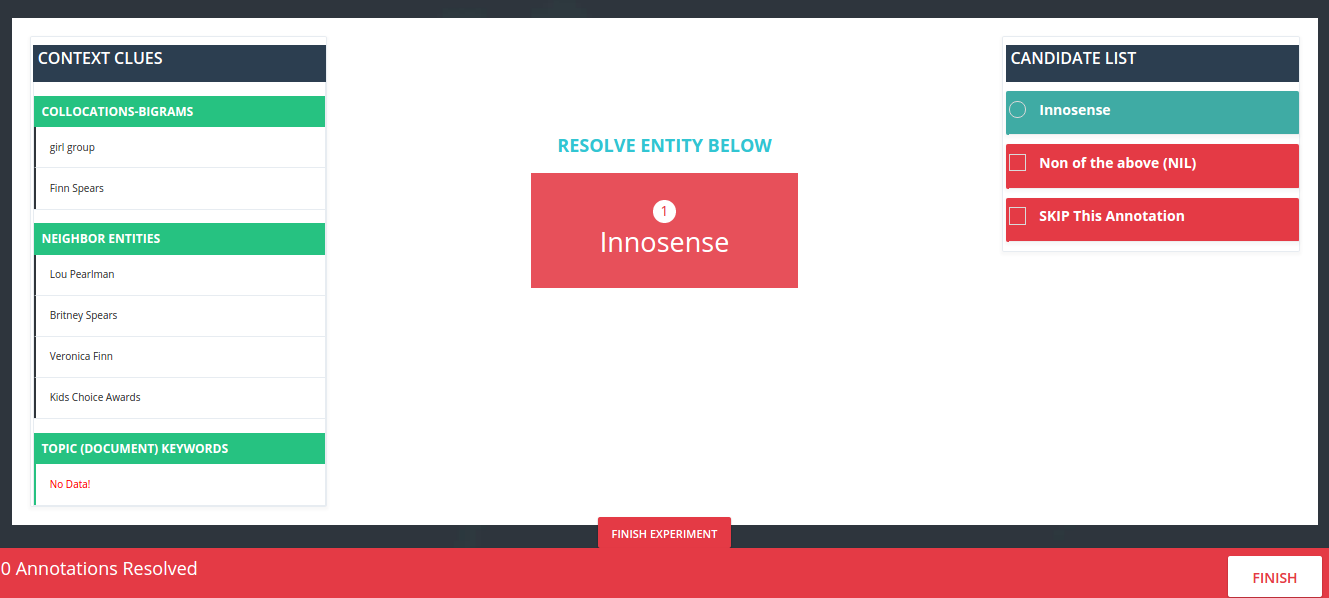
\includegraphics[width=\linewidth]{figures/annotateme-interface.png}
  \caption{The AnnotateMe Interface used to conduct the first experiment for validating the links generated by the NED Framework}
  \label{fig:annotateme-interface}
\end{figure}

During the implementation of the AnnotateMe Interface, we tried to come up with a simple UI and UX design of the interface in order to maintain low levels of complexity and avoiding confusion. Some of the design patterns identified by Hinze et al. \cite{15} necessary for non-expert users to annotate the presented content have been explored while implementing the annotation interface. These design patterns include:
\begin{itemize}
    \item Intuitive User Interface - an interface that is easy to grasp with actions that require minimal effort to discover and perform
    \item Simple Vocabularies - the current architecture of the framework provides annotations of entities within the categories of Organization, Location and People which are genuinely simple in nature.
    \item Focus on user task - The interface does not have any disruptive features or elements that would shift the focus of the annotator from its main task, that is, resolving the presented named entity.
\end{itemize}

% Quality check
According to Bontcheva et al. \cite{33} the single most influential part of any linguistic annotation exercise is the annotators ability to understand and conduct the annotation task. In order to achieve this, the guidelines and tools provided by the annotation interface play a major role in controlling such behavior. Presenting the user with simple, short guidelines that include examples and specific instructions on how to perform certain actions is very helpful. Additionally, having a clean interface is of utter most importance which contributes to an intuitive interaction during the annotation process. \cite{33} 

Figure \ref{fig:annotateme-interface} represents the design of the AnnotateMe Interface used for conducting annotations with non-expert users. The target entity mention to be resolved is presented in the middle of the page and attracts the users focus by reflecting its importance in the overall task. The contextual clues are presented to the right hand side of the interface and are grouped based on their origin of extraction. The right hand side of the interface is reserved for the candidate list. Each candidate can be expanded by clicking on its name. The expanded candidate provides the user with additional information that describes the meaning of the candidate (usually a short description). The two last options in the candidate section highlighted with red provide some degree of freedom to the user in case they are unfamiliar with the entity or when they think that the correct candidate is not provided in the list. These two options being discussed are: \textit{Non of the above(NIL)} and \textit{Skip this annotation}. The interface presented in Figure \ref{fig:annotateme-interface} has been used to conduct the first experiment which will be described in detail in the next upcoming section.